% Definimos el tipo y tamaño de letra
\documentclass[a4paper,times, 12pt]{article}
% Librerías
\usepackage[utf8]{inputenc}
\usepackage[spanish,mexico]{babel}
\setlength{\textwidth}{18cm}
\setlength{\oddsidemargin}{-1cm}
\setlength{\headsep}{-1cm}
\setlength{\voffset}{0cm}
\setlength{\topmargin}{0cm}
\setlength{\headheight}{0cm}
\usepackage{tikz}
\usetikzlibrary{calc,arrows}
\usepackage{multicol}
\usepackage{lipsum} 
%\bibliographystyle{apacite}
\usepackage[spanish]{babel}
\selectlanguage{spanish}
% Se agrega paquetes para cronograma
%\documentclass[tikz]{standalone}
\usepackage{pgfgantt}
\usepackage{hyperref}
\usepackage{cite}

\begin{document}

%%%%%% ENCABEZADO %%%%%%%%%%%%%%%%%%%%%%%%%%%%%%%%%%%%%%%
% Logo de la maestría
\colorbox{white!10!}{
    \begin{minipage}[t]{0.05\textwidth} %0.165 
       \begin{flushright}
        
\includegraphics[width=2in]{logo UPS.png}
       \end{flushright}
    \end{minipage}
    \begin{minipage}[H]{0.62 \textwidth} %0.62
        \begin{center}
         
        \end{center}
    \end{minipage}
    \begin{minipage}[t]{0.05 \textwidth}
        \begin{flushleft}
        \hspace{10.25cm}
            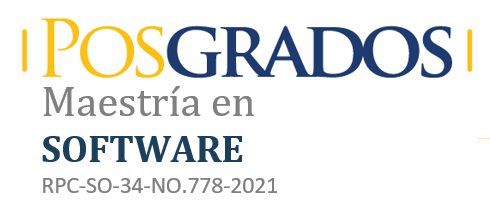
\includegraphics[width=2in]{Posgrados.png}
        \end{flushleft}
    \end{minipage}
}

\begin{tikzpicture}
    \draw[thick] (-6.5,0)--(11.2,0);
\end{tikzpicture}
%%%%%%%%%%%%%%%%%%%%%%%%%%%%%%%%%%%%%%%%%%%%%%%%%%%%%%%%%
\vspace{0.1cm}

\begin{center}
{\large\textsc{ANTEPROYECTO DEL TRABAJO DE TITULACIÓN}} \\
\vspace{0.5cm}
{ \large \textbf{Eduardo Guillermo Aguilar Riera}} \\ 
\vspace{0.25cm}
{ \large \textbf{Juan Gabriel Naula Sanisaca}}
\end{center}

\vspace{0.1cm}

\section{Tema del Trabajo de Titulación:  }
\begin{center}
Aplicación de principios DevOps y metodologías ágiles para el desarrollo del Módulo del Historial financiero de la COAC Jardín Azuayo.
\end{center}
\section{Docente tutor propuesto:   }
\begin{center}
Msc. Cintya Aguirre
\end{center}
\section{Antecedentes:}
\subsection{DevOps}
A principios de la década del 2000, el desarrollo de software y la gestión de operaciones eran dos mundos separados donde desarrollo parecía ser visto como estratégico y operaciones fue vista como tácticas a menudo delegado o subcontratado por completo. Por un lado, los desarrolladores se enfocaban en escribir el código y operaciones se centraban en mantener disponible el servicio para los clientes \cite{kim2016devops}.
A raíz de esta realidad el proceso de desarrollo se encontraba comprometido con tiempos incumplidos, grandes versiones de software, trabajo descoordinado, donde la entrega de valor se podía ver solo al finalizar el proyecto con lo cual los errores solo se podían palpar al finalizar el mismo y los costos para corregir la deuda técnica existente eran muy costosos cite\cite{kim2016devops}. Así mismo una vez culminado el proceso de desarrollo de software vendrían nuevos dolores de cabeza ya que el despliegue de cada versión podrían causar un inmenso caos e interrupción del servicio por el proceso manual de despliegue con lo cual acarrearían a grandes sanciones por la afección directa que esto representaba en el cliente \cite{kim2016devops}.

 Sin embargo mientras se investigaba los criterios de pruebas de aplicaciones un grupo de trabajo encontró conceptos inspirados con la metodología ágil, como el desarrollo guiado por pruebas y Scrum \cite{4599477}

En la continua busca de soluciones a los constantes errores en el proceso de desarrollo de software aparece conceptos inspirados con metodología Ágil con lo cual se implementan en el desarrollo por Sprint que permitiría realizar pequeñas entregas y mejoras constantes, permitiendo la interacción y una mejor comprensión de las necesidades de los clientes \cite{4599477}. Con la entrega del primer sprint daría paso al despliegue del aplicativo lo cual desencadena una nueva necesidad de la configuración correcta de los servidor por parte de Operaciones TI el mismo que en base a prueba error permitiría una solución y mejora continua \cite{4599477}.
Con base a estas premisas empieza el proceso de madurez con la formación de equipos de trabajo multidisciplinarios, priorizaciones, seguimientos a cambios, herramientas e integración que hoy se define como DevOps nombre acuñado en Ágile Conference 2008 por el autor Patrick Debois \cite{4599477}.
 
 DevOps es un conjunto de buenas prácticas que busca generar una estrecha colaboración entre propietarios de productos, arquitectura, desarrollo, control de calidad, operaciones de TI y seguridad de la información para lograr objetivos comunes donde el trabajo mancomunado aporte al ciclo de vida del desarrollo de software \cite{kim2016devops}.
DevOps busca generar ese cambio de cultura y una comunicación efectiva entre el equipo, lo cual permitirá tener una comprensión más profunda de las necesidades del cliente que permita acelerar la entrega productos de software de alta calidad al automatizar los procesos \cite{4599477}.

DevOps se basa en principios como la automatización, integración continua y despliegue continuo, es busca de acelerar el proceso, garantizando estabilidad, eficiencia, confiabilidad, disponibilidad y seguridad \cite{AZAD2023107150}.

DevOps busca la colaboración como equipo a la hora de brindar soluciones y en la entrega de cambios, requerimientos y actualización de software \cite{AZAD2023107150}. 


% Como se ha aplicado en finanzas (Devops on finance)
\subsection{DevOps en las finanzas} 
La aplicación de DevOps en la industria financiera al igual que el mundo de la tecnología en línea es altamente competitivo y es muy importante el crecimiento continuo y el cumplimiento de objetivos a corto plazo \cite{bird2017devops}.
Los servicios financieros pueden recurrir a DevOps en busca de formas de introducir nuevos productos y servicios más rápido, pero al mismo tiempo necesitan trabajar dentro de las limitaciones para cumplir con estrictos tiempos de actividad y rendimiento \cite{bird2017devops}.
La adopción de DevOps en la industria financiera plantea importantes desafíos y costos elevados. Pero los beneficios son demasiado grandes para ignorarlos al igual de los riegos de no entregar valor a los clientes con la suficiente rapidez y perderlos frente a los competidores, especialmente frente a empresas disruptivas en línea impulsadas por DevOps \cite{bird2017devops}.

Las ideas y principios agiles (priorizar el software sobre la documentación, la entrega frecuente, la colaboración cara a cara y un enfoque en la excelencia técnica y la automatización) forman la base de DevOps. Y la entrega continua que es el marco de control para DevOps, también se basa en una práctica fundamental de desarrollo ágil: la integración continua donde los desarrolladores se aseguran de que el código crece y se ejecuta correctamente cada vez que se registra un cambio, la entrega continua lleva esto al siguiente paso \cite{bird2017devops}.
La entrega continua busca en aprovisionar o configurar entornos de pruebas para que coincidan en lo posible con la producción de forma automática; empaquetar el código e implementarlo en entornos de pruebas automáticamente, ejecutar pruebas de aceptación pruebas de estrés, pruebas de rendimiento y pruebas de seguridad con el fin de   que el sistema esté siempre listo para implementarlo en producción \cite{bird2017devops}.
DevOps comparte la responsabilidad de monitorear el sistema entre los equipos de operaciones y desarrollo exponiendo métricas de producción registro de excepciones y alerta a los desarrolladores \cite{bird2017devops}.



% Como se ha aplicado en empresa
\subsection{DevOps nivel empresarial}
Una de las falencias principales en el contexto empresarial que no se tiene es esta estrecha relación entre el equipo de Desarrolladores y Operaciones lo cual retrasa y afecta al cliente en la implementación de nuevos productos y soluciones a incidencias generadas en ambientes productivos. Cabe mencionar que actualmente es necesaria la implementación de herramientas que apalanquen en el proceso de entrega y despliegue continuo de manera automático.

% Principios agiles
\subsection{Principios Ágil}
En el pasado, los proyectos de desarrollo de software solían demandar años de planificación antes de que se iniciara la programación, lo que a menudo resultaba en costosos desastres. Era común la necesidad de rehacer completamente el software después de invertir sumas significativas de dinero. Para abordar estos desafíos, en el año 2001, un grupo de 17 personas se reunió para discutir las técnicas y procesos de desarrollo de software. Fue durante esta reunión que se acuñó el término 'Metodologías Ágiles' para describir los nuevos enfoques que estaban emergiendo como alternativas a los métodos tradicionales, los cuales se caracterizaban por ser excesivamente rígidos y depender en gran medida de una planificación exhaustiva antes de iniciar el proceso.

Para ello firmaron el Manifiesto Ágil, el cual se basa en los siguientes principios: Individuos e interacciones sobre procesos y herramientas, Software funcionando sobre documentación extensiva, Colaboración con el cliente sobre negociación contractual, respuesta ante el cambio sobre seguir un plan.

En base a los principios anteriormente descritos han surgido una serie de marcos de trabajo y/o metodologías, entre las principales y más usadas se encuentra Scrum, tal como lo indican algunos autores, Scrum es un marco de trabajo liviano que ayuda a las personas, equipos y organizaciones a generar valor a través de soluciones adaptativas para problemas complejos \cite{schwaber2020guia}.

Finalmente, según sus autores, Scrum se basa en el empirismo y el pensamiento Lean, el empirismo afirma que el conocimiento proviene de la experiencia y de la toma de decisiones con base en lo observado, mientras que el pensamiento Lean reduce el desperdicio y se enfoca en lo esencial \cite{schwaber2020guia}.


% y como todo esto genera una necesidad.
\subsection{Necesidad}
DevOps hoy en día es parte fundamental y necesaria en el proceso de desarrollo de software de la Cooperativa y empresas tecnológicas ya que permite reducir los tiempos dolorosos de respuesta y comprensión efectiva de las necesidades reales en la entrega de productos que generen valor al socio y estos sean integrados y entregados de manera continua con el fin de brindar una mejor experiencia a los socios. 


 %\lipsum[1-1]
       
\section{Justificación:}   

Este trabajo se centrará en llevar a cabo la aplicación de los principios de DevOps (Development / Operations) y metodologías Ágiles en el Módulo Historial financiero siendo este una parte fundamental para la Cooperativa en la toma de decisiones en el proceso de análisis de los socios a la hora de otorgar un Crédito o Línea de Crédito. 
Así pues la aplicación de estos principios permitirá mejorar los tiempos, calidad y la frecuencia de entrega de las productos de software de manera colaborativa mediante el uso de herramientas de automatización que nos permita una integración continua iniciando desde el desarrollo, análisis de código, pruebas e implementación, siendo este hoy en día un aparte esencial de TI, claro está siempre debe estar acompañado de metodologías ágiles que encamine proceso y permita realizar lanzamientos en pequeñas funcionalidades que aporten valor al cliente  y no esperar hasta que se culmine con el desarrollo de todo el software. 
Este trabajo busca mejorar la realidad existente en la cooperativa en cuanto a tiempos muertos en la entrega de soluciones de software que interrumpen el normal funcionamiento de los servicios de TI debido a la falta de experiencia en la organización, procesos, principios, metodologías y automatizaciones.

\section{Objetivos:}
%Presenta el objetivo general del trabajo y los objetivos específicos que se alcanzarán con el desarrollo del mismo. 
\subsection*{Objetivo General:}
Implementación de un modelo CI/CD alineado a la propuesta de valor para el Módulo del Historial Financiero de la COAC Jardín Azuayo.
\subsection*{Objetivos Específicos:}

\begin{itemize}
    \item Definir de manera temprana los requisitos del módulo del Historial Financiero, mediante la utilización de  Lean Inception para definir el mínimo producto viable (MVP) que se implementará en la COAC Jardín Azuayo.

    \item Diseño de prototipos del MVP del módulo del Historial Financiero, en base al Product Backlog, mediante Mockups, para obtener una retroalimentación del usuario con respecto al diseño planteado.
    

    \item Seleccionar las herramientas adecuadas para la implementación de CI/CD, mediante la creación de los pipeline, repositorios de versionamientos, configuración de ambientes de desarrollo, para automatizar las tareas, y lograr un impacto significativo en la eficiencia, la calidad y la agilidad del proceso de desarrollo.

    \item Construcción de un MVP del módulo de historial financiero, mediante la automatización de procesos de: desarrollo, pruebas, seguridades,  para garantizar una automatización efectiva y una entrega continua de software de alta calidad que pueda servir de base para los futuros desarrollos en la cooperativa.

    \item Medir la percepción y satisfacción de los usuarios,
    mediante encuestas de satisfacción, comparación de tiempos de entrega de valor anteriores versus los tiempos actuales aplicando metodologías ágiles, para determinar si los usuarios están satisfechos con el MVP del Historial Financiero entregado y poder obtener una retroalimentación para mejorar para los siguientes sprint. 
    
    
    

\end{itemize}

\section{Alcance:}
\begin{itemize}
    \item Utilizar Scrum como metodología en el proceso de desarrollo de software para entrega de valor al cliente.
    \item Implementar la herramienta Sonarqube para análisis de código estático.
    \item Implementación de pruebas unitarias automatizadas para desarrollo de software.
    \item Utilizar herramienta de CI/CD para el proceso de automatización de acuerdo a las buenas prácticas de DevOps.
    \item Desarrollo de un producto mínimo viable (MVP) de historial financiero para la COAC Jardín Azuayo.
    \item Aplicación de principios DevOps en el flujo de desarrollo de software.
    \item Definición de arquitectura del aplicativo web que permita trabajar en concordancia con DevOps.
    \item Aplicación de metodologías ágiles para la definición del producto y requerimientos funcionales (lean inception)...



     \item Análisis de requisitos: Identificación de las necesidades específicas de los usuarios y la cooperativa en relación con el Módulo del Historial Financiero.

    \item Diseño y planificación: Desarrollo de un plan detallado que incluye la definición de procesos DevOps y la elección de metodologías ágiles adecuadas.

    \item Implementación de DevOps: Establecimiento de prácticas de colaboración entre los equipos de desarrollo y operaciones, automatización de procesos de entrega y despliegue, integración continua, monitoreo y retroalimentación constante.

    \item Implementación de metodologías ágiles: Aplicación de métodos ágiles, como Scrum o Kanban, para gestionar el desarrollo del módulo, incluyendo la creación de sprints, reuniones de revisión y planificación, y ajustes iterativos en función de las necesidades del usuario.

    \item Desarrollo de software: Creación, codificación y prueba de las funcionalidades del Módulo del Historial Financiero.

    \item Pruebas y control de calidad: Ejecución de pruebas funcionales y de rendimiento, asegurando que el software cumpla con los estándares de calidad y funcione conforme a los requisitos.

    \item Implementación y despliegue: Puesta en producción del módulo de manera gradual y controlada, minimizando el impacto en la operación de la cooperativa.

    \item Capacitación y adopción: Entrenamiento del personal de la COAC Jardín Azuayo en las nuevas prácticas y herramientas, y fomento de la adopción de los principios DevOps y metodologías ágiles.

    \item Seguimiento y mejora continua: Establecimiento de métricas de rendimiento y monitoreo constante para identificar oportunidades de mejora y ajustes en los procesos.

    \item Entrega final: Entrega del Módulo del Historial Financiero completamente funcional y adaptado a las necesidades reales de la cooperativa y sus usuarios.
\end{itemize}
\section{Metodología:}

\begin{figure}[h]
    \centering
    %\includegraphics[width=40mm,height=10mm]
    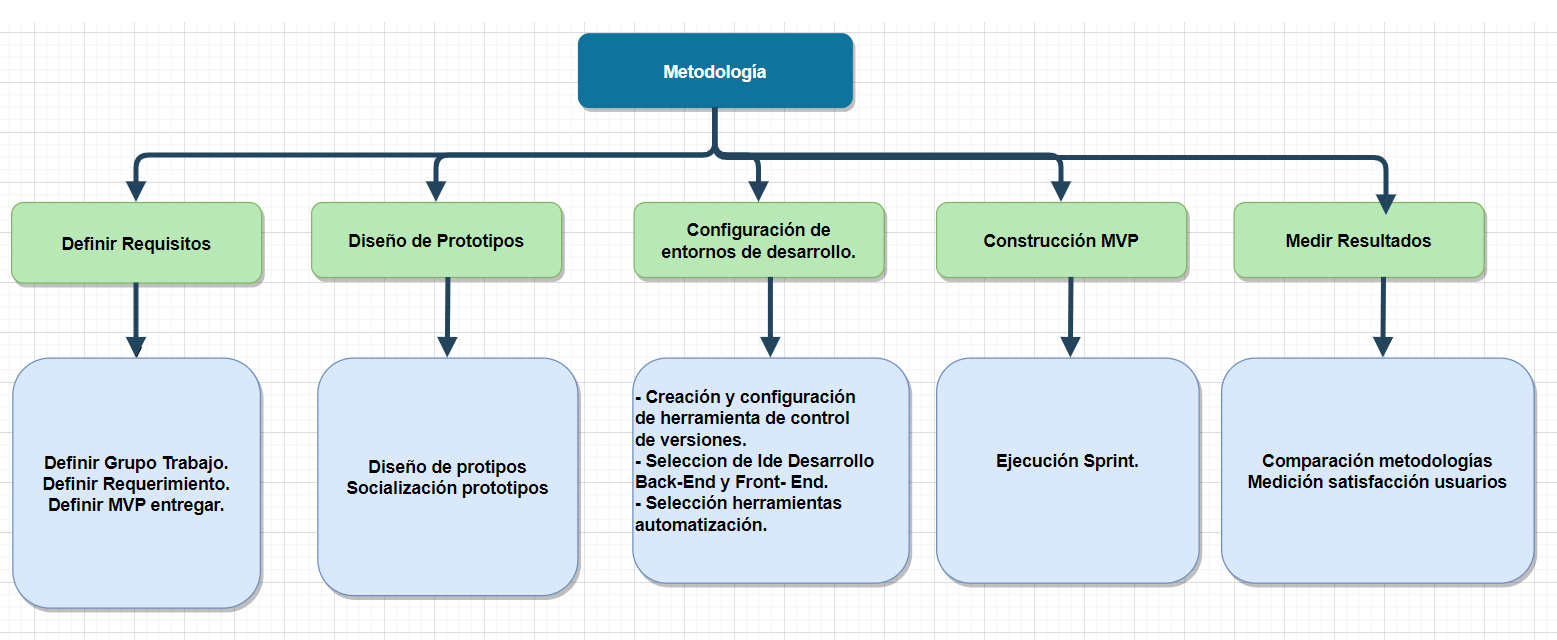
\includegraphics[width=1\textwidth]
    {Metodologia.png}
    \caption{Metodología}
    \label{Fig1:1}
\end{figure}

Definir un proceso DevOps con metodologías agiles en base a la experimentación con el uso de herramientas tecnológicas que permitan construir un MVP que ayude a reducir los tiempos de implementación de soluciones tecnológicas y que sirva como base en la Cooperativa para el desarrollo de los proyectos futuros.

\subsection{Definir Requerimientos}

\begin{itemize}
\item Definir equipo DevOps
Se realizarán reuniones de trabajo con las personas del equipo del core financiero de la COAC Jardín Azuayo, para definir los equipos de trabajo y sus roles de acuerdo a la metodología Scrum, para ello se designarán: Product Owner, Scrum Master y Development Team de acuerdo a las capacidades y aptitudes de cada una de las personas.

\item  Definir alcance
Una vez se logre determinar los problemas que se tiene actualmente con el Historial Financiero de la COAC Jardín Azuayo, se leventarán unas historias de usuario, se crearà un product backlog y se priorizaràn las historias a realizarse en los primeros sprint.

\item Definir MVP
Una vez se tenga priorizado las actividades, se negociará con el equipo Scrum a fin de determinar cuál es el MVP que se podrá entregar para satisfacer las necesidades del Historial Financiero 
\end{itemize}

\subsection{Diseño de Prototipos}
\begin{itemize}
    \item Diseñar prototipos en el contexto de DevOps puede ayudar a visualizar y probar las implementaciones de procesos, flujos de trabajo y herramientas antes de implementarlos completamente, para ello debemos tener claro cuál es el propósito y los objetivos del proyecto DevOps, en este caso nos basaremos en las historias definidas en el producto backlog, posteriormente buscaremos y seleccionaremos una herramienta de prototipado que sea fácil de usar y nos permita trabajar en línea varias personas al mismo tiempo.
    
    \item Se puede utilizar herramientas de diseño o diagramación para crear prototipos visuales de los procesos y flujos de trabajo DevOps, tales como: diagramas de flujo, diagramas de Gantt, diagramas de casos de uso, o herramientas de modelado de procesos.

    \item Finalmente se presentarán los prototipos al equipo Scrum y a los interesados a fin de recopilar comentarios y obtener retroalimentación para identificar posibles mejoras o ajustes en el diseño, con base a los comentarios recibidos se debe iterar el diseño de los prototipos y realizar los ajustes necesarios hasta lograr que los prototipos reflejen de manera precisa cómo funcionará el MVP del Historia Financiero.

\end{itemize}

\subsection{Configuración de entornos de desarrollo.}
\begin{itemize}
    \item Creación y configuración de herramienta de control de versiones:
    Al centrar DevOps su atención en la colaboración entre el equipo de desarrollo y operaciones para automatizar y mejorar el proceso de desarrollo de software, por lo cual en conjunto como el grupo de trabajo se analizara y seleccionara la herramienta de control de versiones más se apegue a la realidad de la cooperativa.
    \item Seleccion de Ide Desarrollo Back-End y Front- End:
    Para este proceso se realizara la selección de herramientas de desarrollo acorde a la arquitectura a implementar en la cooperativa, herramientas tanto para back-end,  front-end, herramientas de Testeo de servicios Rest.
    \item Seleccionar herramientas de automatización y Configuración ambientes.
    \item Selección herramientas automatización.
\end{itemize}

\subsection{Construcción de MVP}

\section{Cronograma de actividades:}
\begin{figure}[h!]
    \centering
    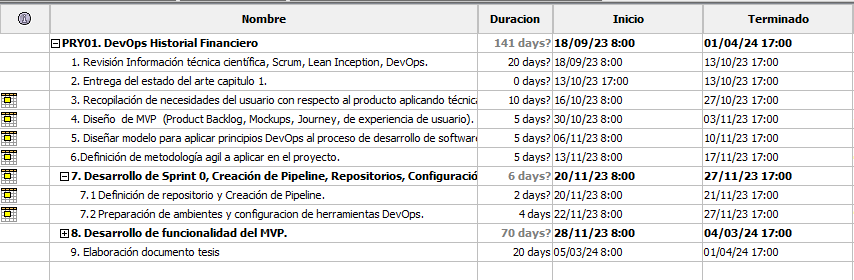
\includegraphics[width=1.0\textwidth]{Cronograma.png}
    \caption{Cronograma}
    \label{Fig1:1}
\end{figure}
%\include{Cronograma}
    

\section{Presupuesto: (Opcional)}

Este apartado incluirá los recursos e información financiera para el Trabajo de Titulación. 

\bibliographystyle{apalike}
\bibliography{State_art_DevOps_Architecture}

\end{document}
%\vspace{1cm}
%Este apartado contiene el listado de referencias empleadas %para la elaboración del documento, de preferencia en %formato APA u otros formatos Preconocidos.


